\chapter{Implementacija i korisničko sučelje}
		
		
		\section{Korištene tehnologije i alati}
		
			 Za međusobnu komunikaciju tijekom izrade naše KuhajIT aplikacije korištene su dvije aplikacije: \textcolor{blue}{\underline{\href{https://discord.com/download}{\textcolor{blue}{Discord}}}}\footnote{\url{https://discord.com/download}} i \textcolor{blue}{\underline{\href{https://www.whatsapp.com/download/}{\textcolor{blue}{WhatsApp}}}}\footnote{\url{https://www.whatsapp.com/download/}}.
			 		 
WhatsApp je aplikacija za razmjenu poruka koja omogućava korisnicima slanje tekstualnih poruka, medijskih datoteka (poput slika, videa i audio zapisa), te poziva i video poziva putem internetskog povezivanja. Mi smo ju koristili za interno dogovaranje o onome što je iduće potrebno obaviti te o terminima sastanaka uživo.

Discord je platforma za komunikaciju putem interneta koja je prvobitno dizajnirana za zajednice igrača, ali se brzo proširila na različite druge vrste korisnika. Omogućava korisnicima stvaranje privatnih ili javnih "servera" (prostorija) gdje se mogu razgovarati putem teksta, glasa ili videa. Mi smo ju koristili za hitne sastanke u slučaju da je netko od članova pri izradi naišao na problem bilo kakve vrste i trebala mu je asistencija drugog člana tima.

Upravljanje izvornim kodom ostvareno je sustavom \textcolor{blue}{\underline{\href{https://git-scm.com/downloads}{\textcolor{blue}{Git}}}}\footnote{\url{https://git-scm.com/downloads}}, a udaljeni repozitorij
čitavog projekta dostupan nam je bio na web platformi \textcolor{blue}{\underline{\href{https://github.com/}{\textcolor{blue}{GitHub}}}}\footnote{\url{https://github.com/}}.

			Git je sustav za upravljanje verzijama koji se široko koristi u razvoju softvera. Omogućava programerima i timovima praćenje promjena u izvornom kodu tijekom vremena, praćenje različitih verzija projekta te suradnju među programerima, te smo ga mi na taj način koristili.
			
			GitHub je web platforma za upravljanje verzijama i suradnju na razvoju softvera. Osnovna funkcionalnost GitHub-a leži u Git-u, koji omogućuje razvojnom timu praćenje promjena u izvornom kodu tijekom vremena. 
			Za izradu svih UML dijagrama korišten je alat \textcolor{blue}{\underline{\href{https://astah.net/downloads/}{\textcolor{blue}{Astah UML}}}}\footnote{\url{https://astah.net/downloads/}}.
			
Astah UML je vrsta alata koji pomaže programerima, analitičarima sustava i drugima da vizualiziraju, modeliraju i dokumentiraju arhitekturu softvera. Podržava različite vrste dijagrama, od kojih smo mi koristili dijagrame razreda, stanja, aktivnosti, komponenti, dijagrame obrazaca uporabe te sekvencijske dijagrame.

Odabrana razvojna okruženja pri izradi naše aplikacije bila su \textcolor{blue}{\underline{\href{https://code.visualstudio.com/Download}{\textcolor{blue}{Visual Studio Code}}}}\footnote{\url{https://code.visualstudio.com/Download}} za frontend i \textcolor{blue}{\underline{\href{https://www.eclipse.org/downloads/}{\textcolor{blue}{Eclipse}}}}\footnote{\url{https://www.eclipse.org/downloads/}} za backend.


Visual Studio Code je razvojno okruženje za pisanje koda razvijen od strane Microsofta. Odlikuje ga bogata podrška za web tehnologije, kao što su HTML, CSS, JavaScript, Typescript itd.

Eclipse je razvojno okruženje koje podržava brojne programske jezike, a neki od njih su: Java, C++, PHP, Python, Ruby...

Kako je već prije navedeno, za razvoj frontenda naše aplikacije koristili smo \textcolor{blue}{\underline{\href{https://www.javascript.com/}{\textcolor{blue}{Javascript}}}}\footnote{\url{https://www.javascript.com/}} i \textcolor{blue}{\underline{\href{https://react.dev/}{\textcolor{blue}{React}}}}\footnote{\url{https://react.dev/}}.

JavaScript je visokoprogamski jezik koji se često koristi za izgradnju dinamičkih web stranica i web aplikacija, razvijen u Netscape Communications Corporation-u. Najčešće se koristi za programiranje na strani klijenta.

React je JavaScript biblioteka za izgradnju korisničkih sučelja, koju karakterizira komponentna arhitektura koja olakšava organizaciju koda i upravljanje stanjem aplikacije.

Za razvoj backenda naše aplikacije korišten je \textcolor{blue}{\underline{\href{https://spring.io/projects/spring-boot/}{\textcolor{blue}{Spring Boot}}}}\footnote{\url{https://spring.io/projects/spring-boot/}}.

Spring Boot je open-source okvir za izgradnju Java web aplikacija i mikroservisa, dio šireg Spring ekosustava. Posebno je fokusiran na pojednostavljenje konfiguracije, ubrzanje razvoja i olakšavanje izgradnje samostalnih aplikacija.


			\eject 
			
			
			
		
	
		\section{Ispitivanje programskog rješenja}
			
			\textbf{\textit{dio 2. revizije}}\\
			
			 \textit{U ovom poglavlju je potrebno opisati provedbu ispitivanja implementiranih funkcionalnosti na razini komponenti i na razini cijelog sustava s prikazom odabranih ispitnih slučajeva. Studenti trebaju ispitati temeljnu funkcionalnost i rubne uvjete.}
	
			
			\subsection{Ispitivanje komponenti}
			\textit{Potrebno je provesti ispitivanje jedinica (engl. unit testing) nad razredima koji implementiraju temeljne funkcionalnosti. Razraditi \textbf{minimalno 6 ispitnih slučajeva} u kojima će se ispitati redovni slučajevi, rubni uvjeti te izazivanje pogreške (engl. exception throwing). Poželjno je stvoriti i ispitni slučaj koji koristi funkcionalnosti koje nisu implementirane. Potrebno je priložiti izvorni kôd svih ispitnih slučajeva te prikaz rezultata izvođenja ispita u razvojnom okruženju (prolaz/pad ispita). }
			
			
			
			\subsection{Ispitivanje sustava}
			
			 \textit{Potrebno je provesti i opisati ispitivanje sustava koristeći radni okvir Selenium\footnote{\url{https://www.seleniumhq.org/}}. Razraditi \textbf{minimalno 4 ispitna slučaja} u kojima će se ispitati redovni slučajevi, rubni uvjeti te poziv funkcionalnosti koja nije implementirana/izaziva pogrešku kako bi se vidjelo na koji način sustav reagira kada nešto nije u potpunosti ostvareno. Ispitni slučaj se treba sastojati od ulaza (npr. korisničko ime i lozinka), očekivanog izlaza ili rezultata, koraka ispitivanja i dobivenog izlaza ili rezultata.\\ }
			 
			 \textit{Izradu ispitnih slučajeva pomoću radnog okvira Selenium moguće je provesti pomoću jednog od sljedeća dva alata:}
			 \begin{itemize}
			 	\item \textit{dodatak za preglednik \textbf{Selenium IDE} - snimanje korisnikovih akcija radi automatskog ponavljanja ispita	}
			 	\item \textit{\textbf{Selenium WebDriver} - podrška za pisanje ispita u jezicima Java, C\#, PHP koristeći posebno programsko sučelje.}
			 \end{itemize}
		 	\textit{Detalji o korištenju alata Selenium bit će prikazani na posebnom predavanju tijekom semestra.}
			
			\eject 
		
		
		\section{Dijagram razmještaja}
			
		
		Na slici 5.1 prikazan je dijagram razmještaja. Dijagrami razmještaja prikazuju fizičku arhitekturu programskog sustava, prikazujući razmještaj programskih artefakata na sklopovskim čvorovima ili virtualnim okruženjima. Glavna svrha dijagrama razmještaja u programskom inženjerstvu je pružiti razumijevanje arhitekture razmještaja sustava.
		
		Naš dijagram razmještaja sastoji se od dvije glavne komponente: računalo korisnika i poslužiteljsko računalo. Na računalu korisnika, on putem web preglednika pristupa aplikaciji KuhajIT. Komunikacija između računala korisnika i poslužiteljskog računala uspostavlja se i odvija pomoću protokola HTTP. Unutar poslužiteljskog računala razlikujemo dvije podkomponente: web poslužitelj i poslužitelj baze podataka.
		
					\begin{figure}[H]
			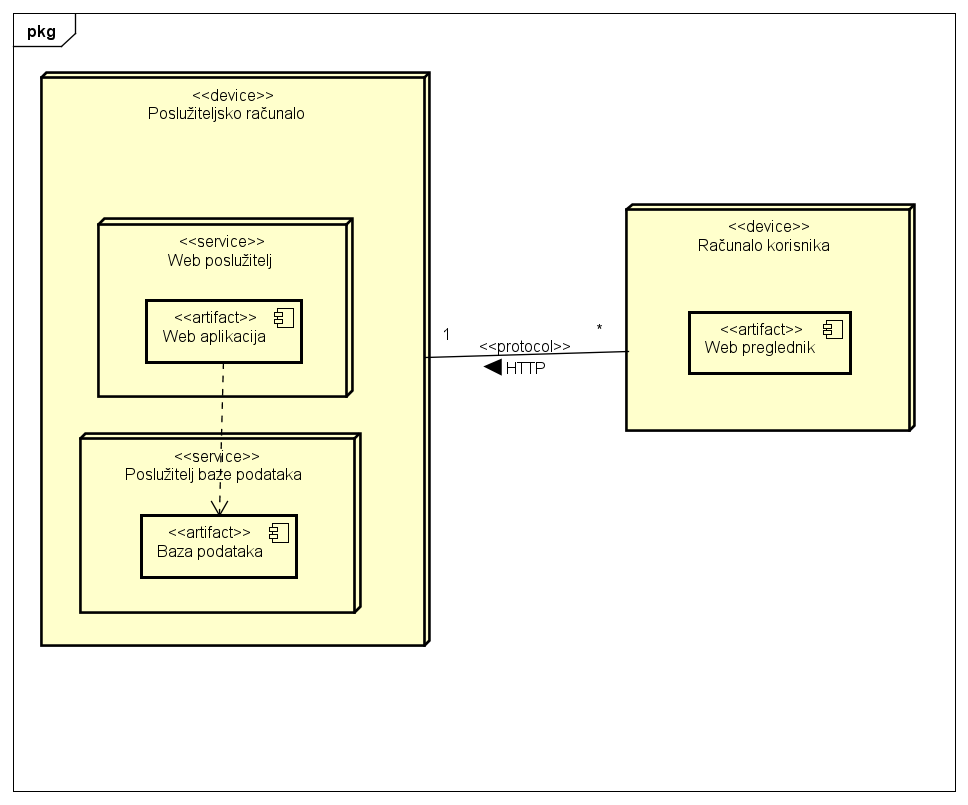
\includegraphics[scale=0.4]{dijagrami/UML_dijagram_razmjestaja.PNG} %veličina slike u odnosu na originalnu datoteku i pozicija slike
			\centering
			\caption{Dijagram razmještaja}
			\label{Dijagram razmještaja}
		\end{figure}
		
		

			\eject 
		
		\section{Upute za puštanje u pogon}
		Naša KuhajIT web-aplikacija, razvijena u okviru ovog projekta, puštena je u pogon putem web platforme  \textcolor{blue}{\underline{\href{https://render.com/}{\textcolor{blue}{Render}}}}\footnote{\url{https://render.com/}}. Render je platforma koja pruža usluge za deploy, hosting i skaliranje web aplikacija, servisa i web stranica. Ističe se jednostavnošću upotrebe, brzim implementacijama i podrškom za različite jezike i okvire, i upravo smo ju zbog tog razloga i odabrali za tzv. deploy. Na Render-u je postavljen Spring Boot poslužitelj, kojega smo spremili u Docker kontejner, a koji odgovara na upite korisnika i statička stranica, koja služi za prikaz React web aplikacije. Ispod je priložena slika komponenata postavljenih na Render.
		
		
			\begin{figure}[H]
			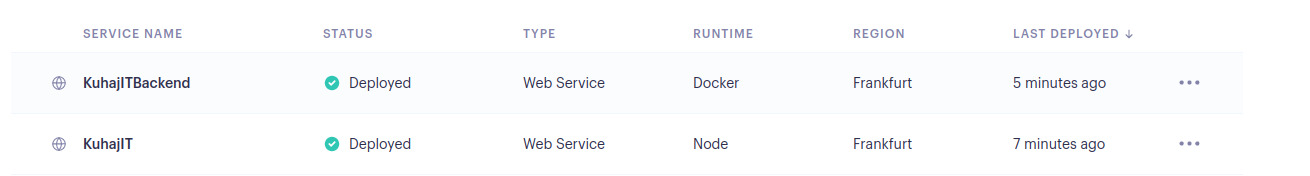
\includegraphics[scale=0.3]{slike/Render_OVERVIEW.JPG} %veličina slike u odnosu na originalnu datoteku i pozicija slike
			\centering
			\caption{Pregled prenesenih komponenti}
			\label{Pregled prenesenih komponenti}
		\end{figure}
		
		\textbf{Postavljanje Spring Boot poslužitelja} \\
		Dio razloga zbog kojeg smo odabrali baš Render za deploy je jednostavnost postavljanja komponenti na njega. Tako je bilo i s postavljanjem Spring Boot poslužitelja koji komunicira sa React aplikacijom, spremljenom u \textcolor{blue}{\underline{\href{https://docker.com/}{\textcolor{blue}{Docker}}}}\footnote{\url{https://docker.com/}} "kontejner". Korištenje Docker-a nam je uvelike olakšalo cijeli proces deploy-a, jer Docker nudi izolirane okoline, zvane kontejnerima, koje sadrže sve potrebno za pokretanje aplikacije, stoga se nije potrebno oslanjati na ono što je instalirano na Render poslužitelju. Na slici ispod prikazan je kod Dockerfile-a. Dockerfile je dokument koji sadrži sve naredbe koje bi se trebale pozvati u naredbenom retku kako bi se aplikacija ispravno i cjelovito pokrenula.
		
		\begin{figure}[H]
			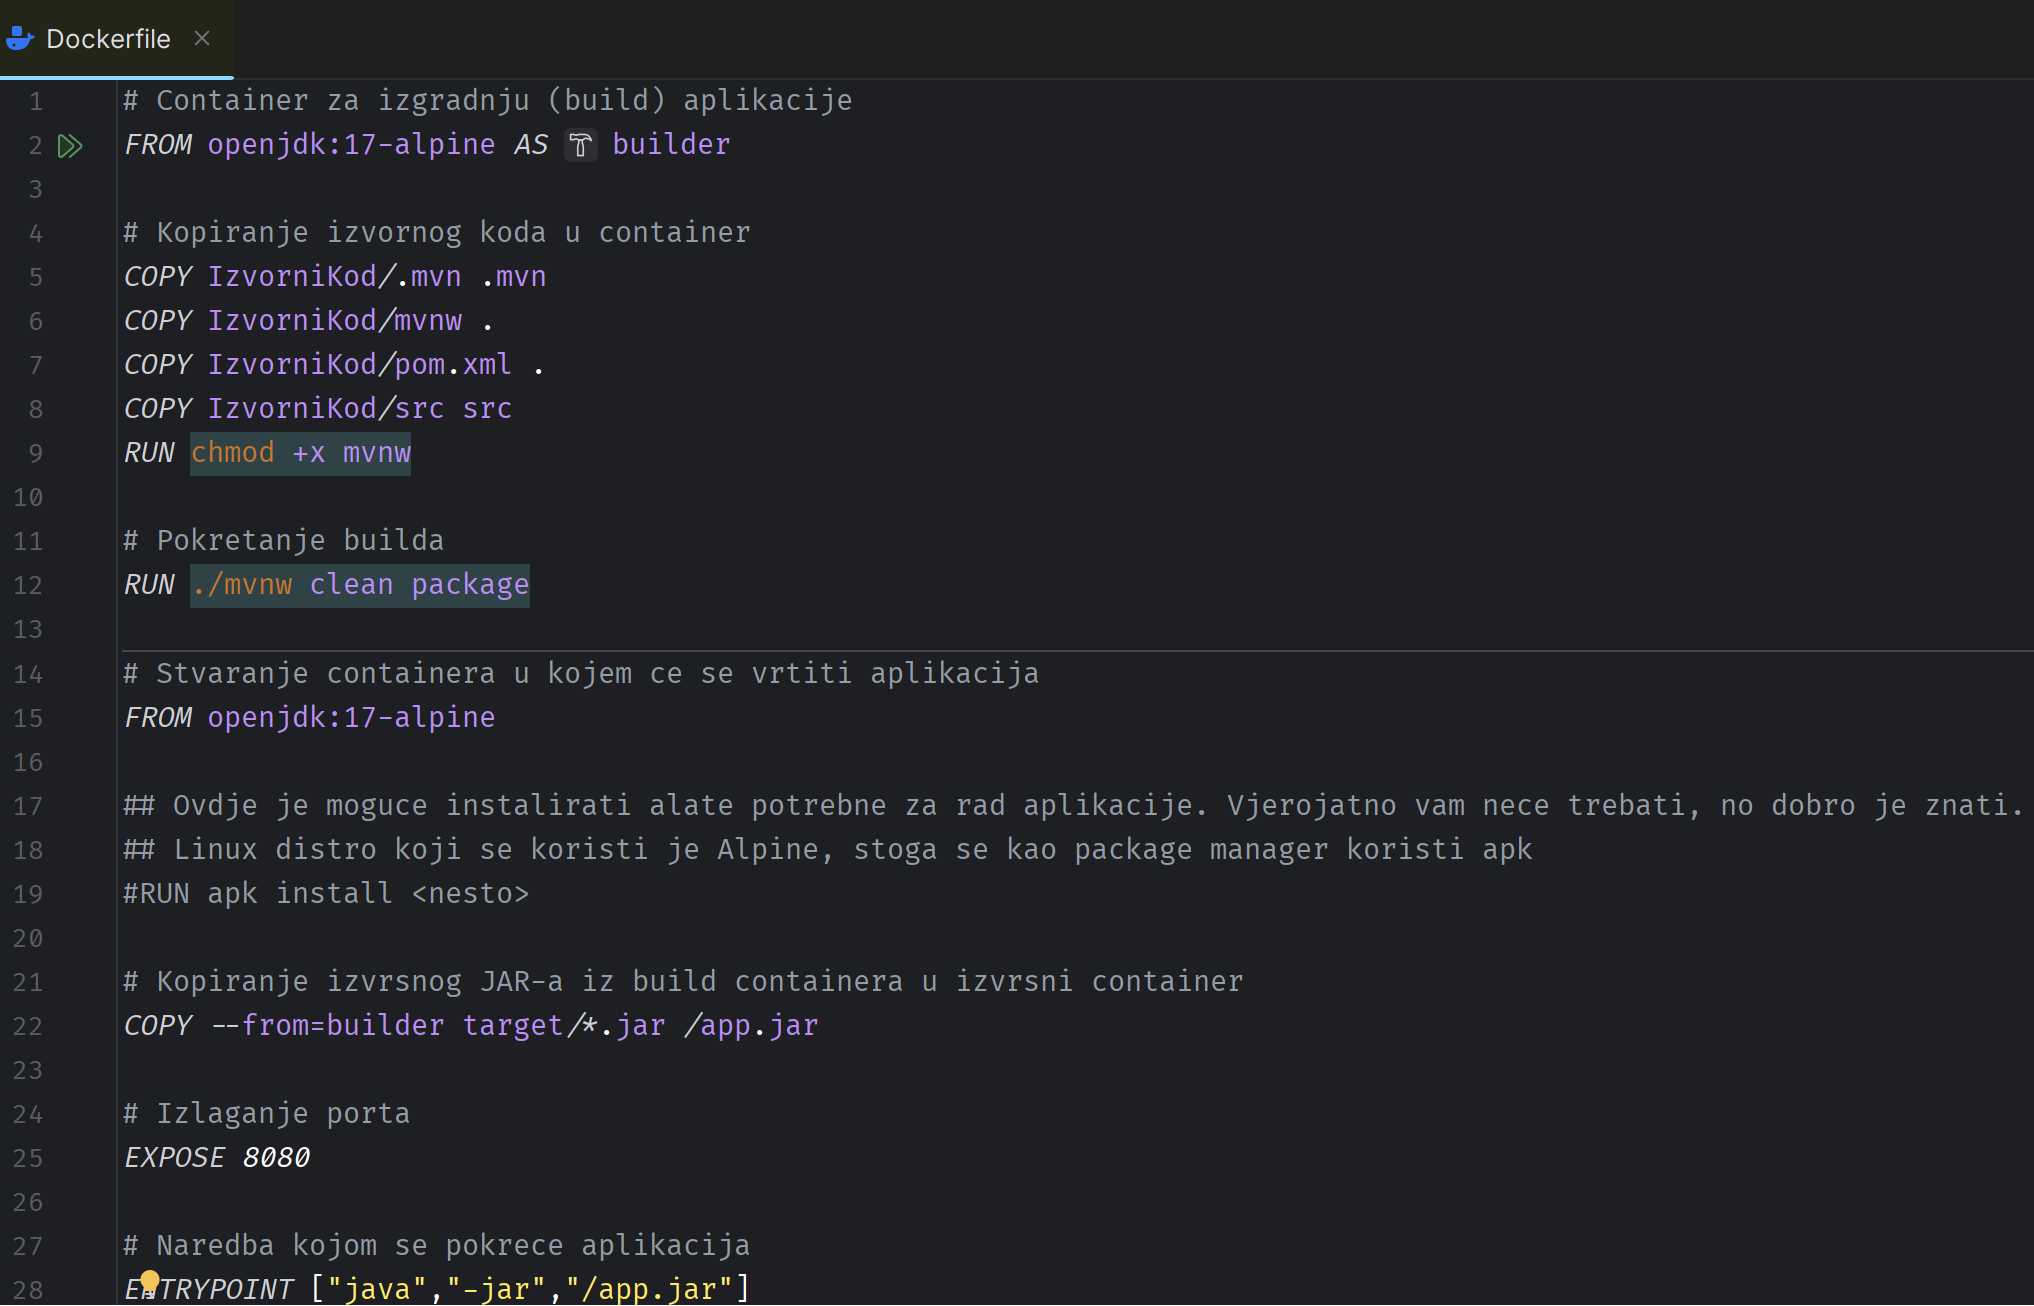
\includegraphics[scale=0.4]{slike/Dockerfile.PNG} %veličina slike u odnosu na originalnu datoteku i pozicija slike
			\centering
			\caption{Dockerfile}
			\label{Dockerfile}
		\end{figure}
		
		
Na početku, potrebno je u gornjem desnom kutu web platforme Render odabrati opciju New, kako je prikazano na slici ispod.
		
			\begin{figure}[H]
			
\includegraphics[scale=0.4]{slike/Render_NEW.PNG} %veličina slike u odnosu na originalnu datoteku i pozicija slike
			\centering
			\caption{Dodavanje nove komponente}
			\label{Dodavanje nove komponente}
		\end{figure}
		
		Zatim, u izborniku koji se prikaže, potrebno je odabrati opciju Web Service, kako je prikazano na slici ispod.
					\begin{figure}[H]
			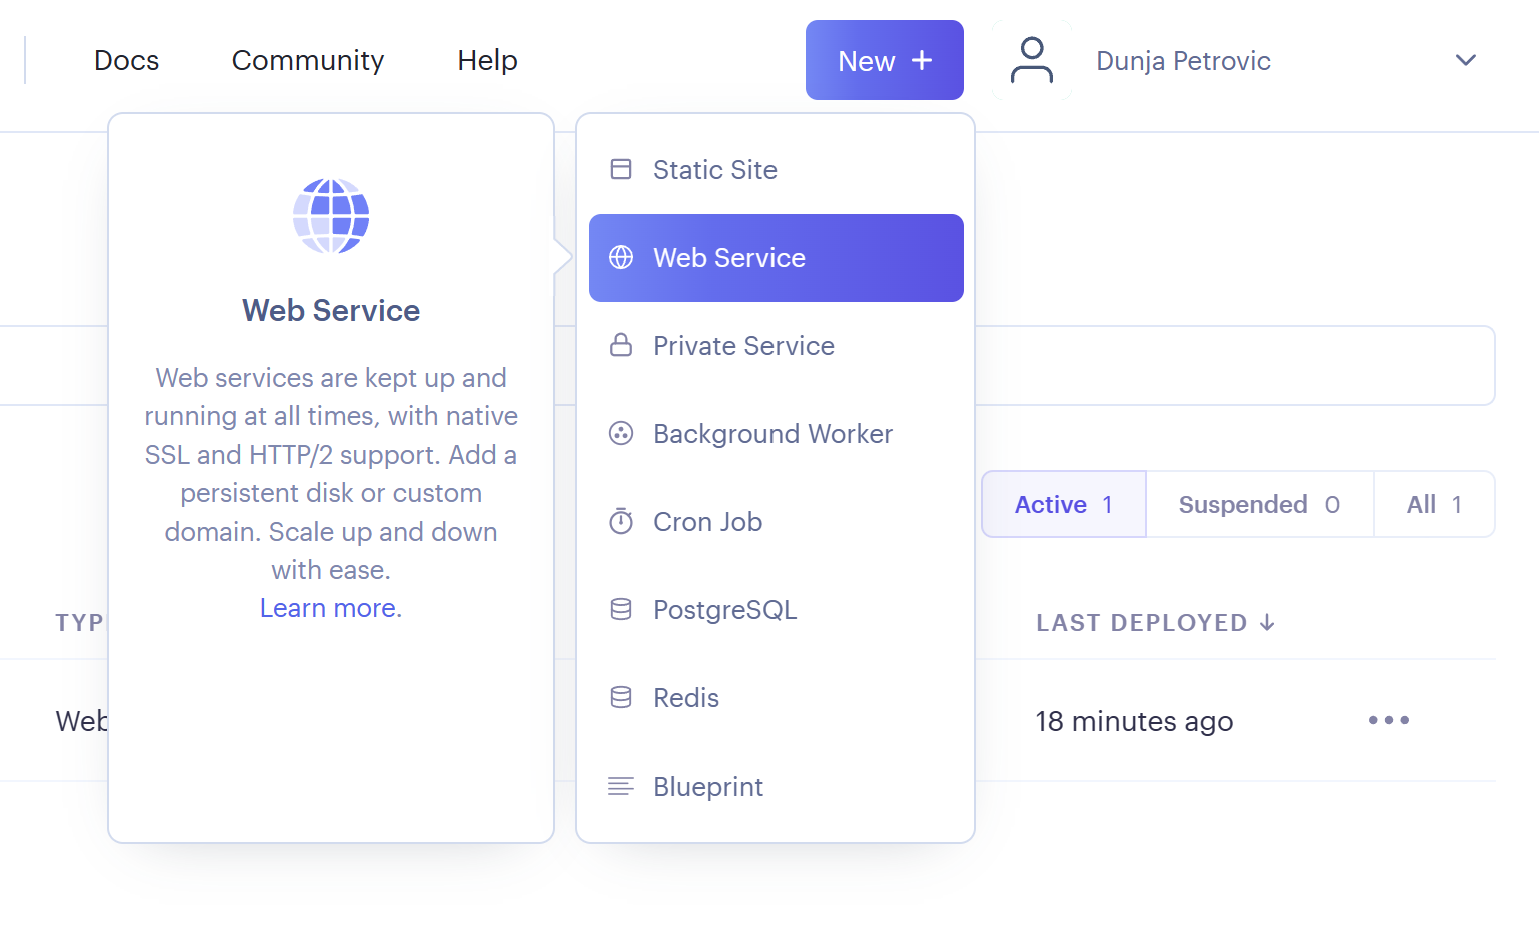
\includegraphics[scale=0.4]{slike/Render_WEB_SERVICE.PNG} %veličina slike u odnosu na originalnu datoteku i pozicija slike
			\centering
			\caption{Odabir opcije Web Service}
			\label{Odabir opcije Web Service}
		\end{figure}
		
		Kada nam se otvori stranica za dodavanje nove komponente tipa "Web Service", nudi nam se opcija odabira GitHub repozitorija iz koje želimo dodati komponentu, koju je potrebno i označiti, kako je prikazano na slici ispod.
		
			\begin{figure}[H]
			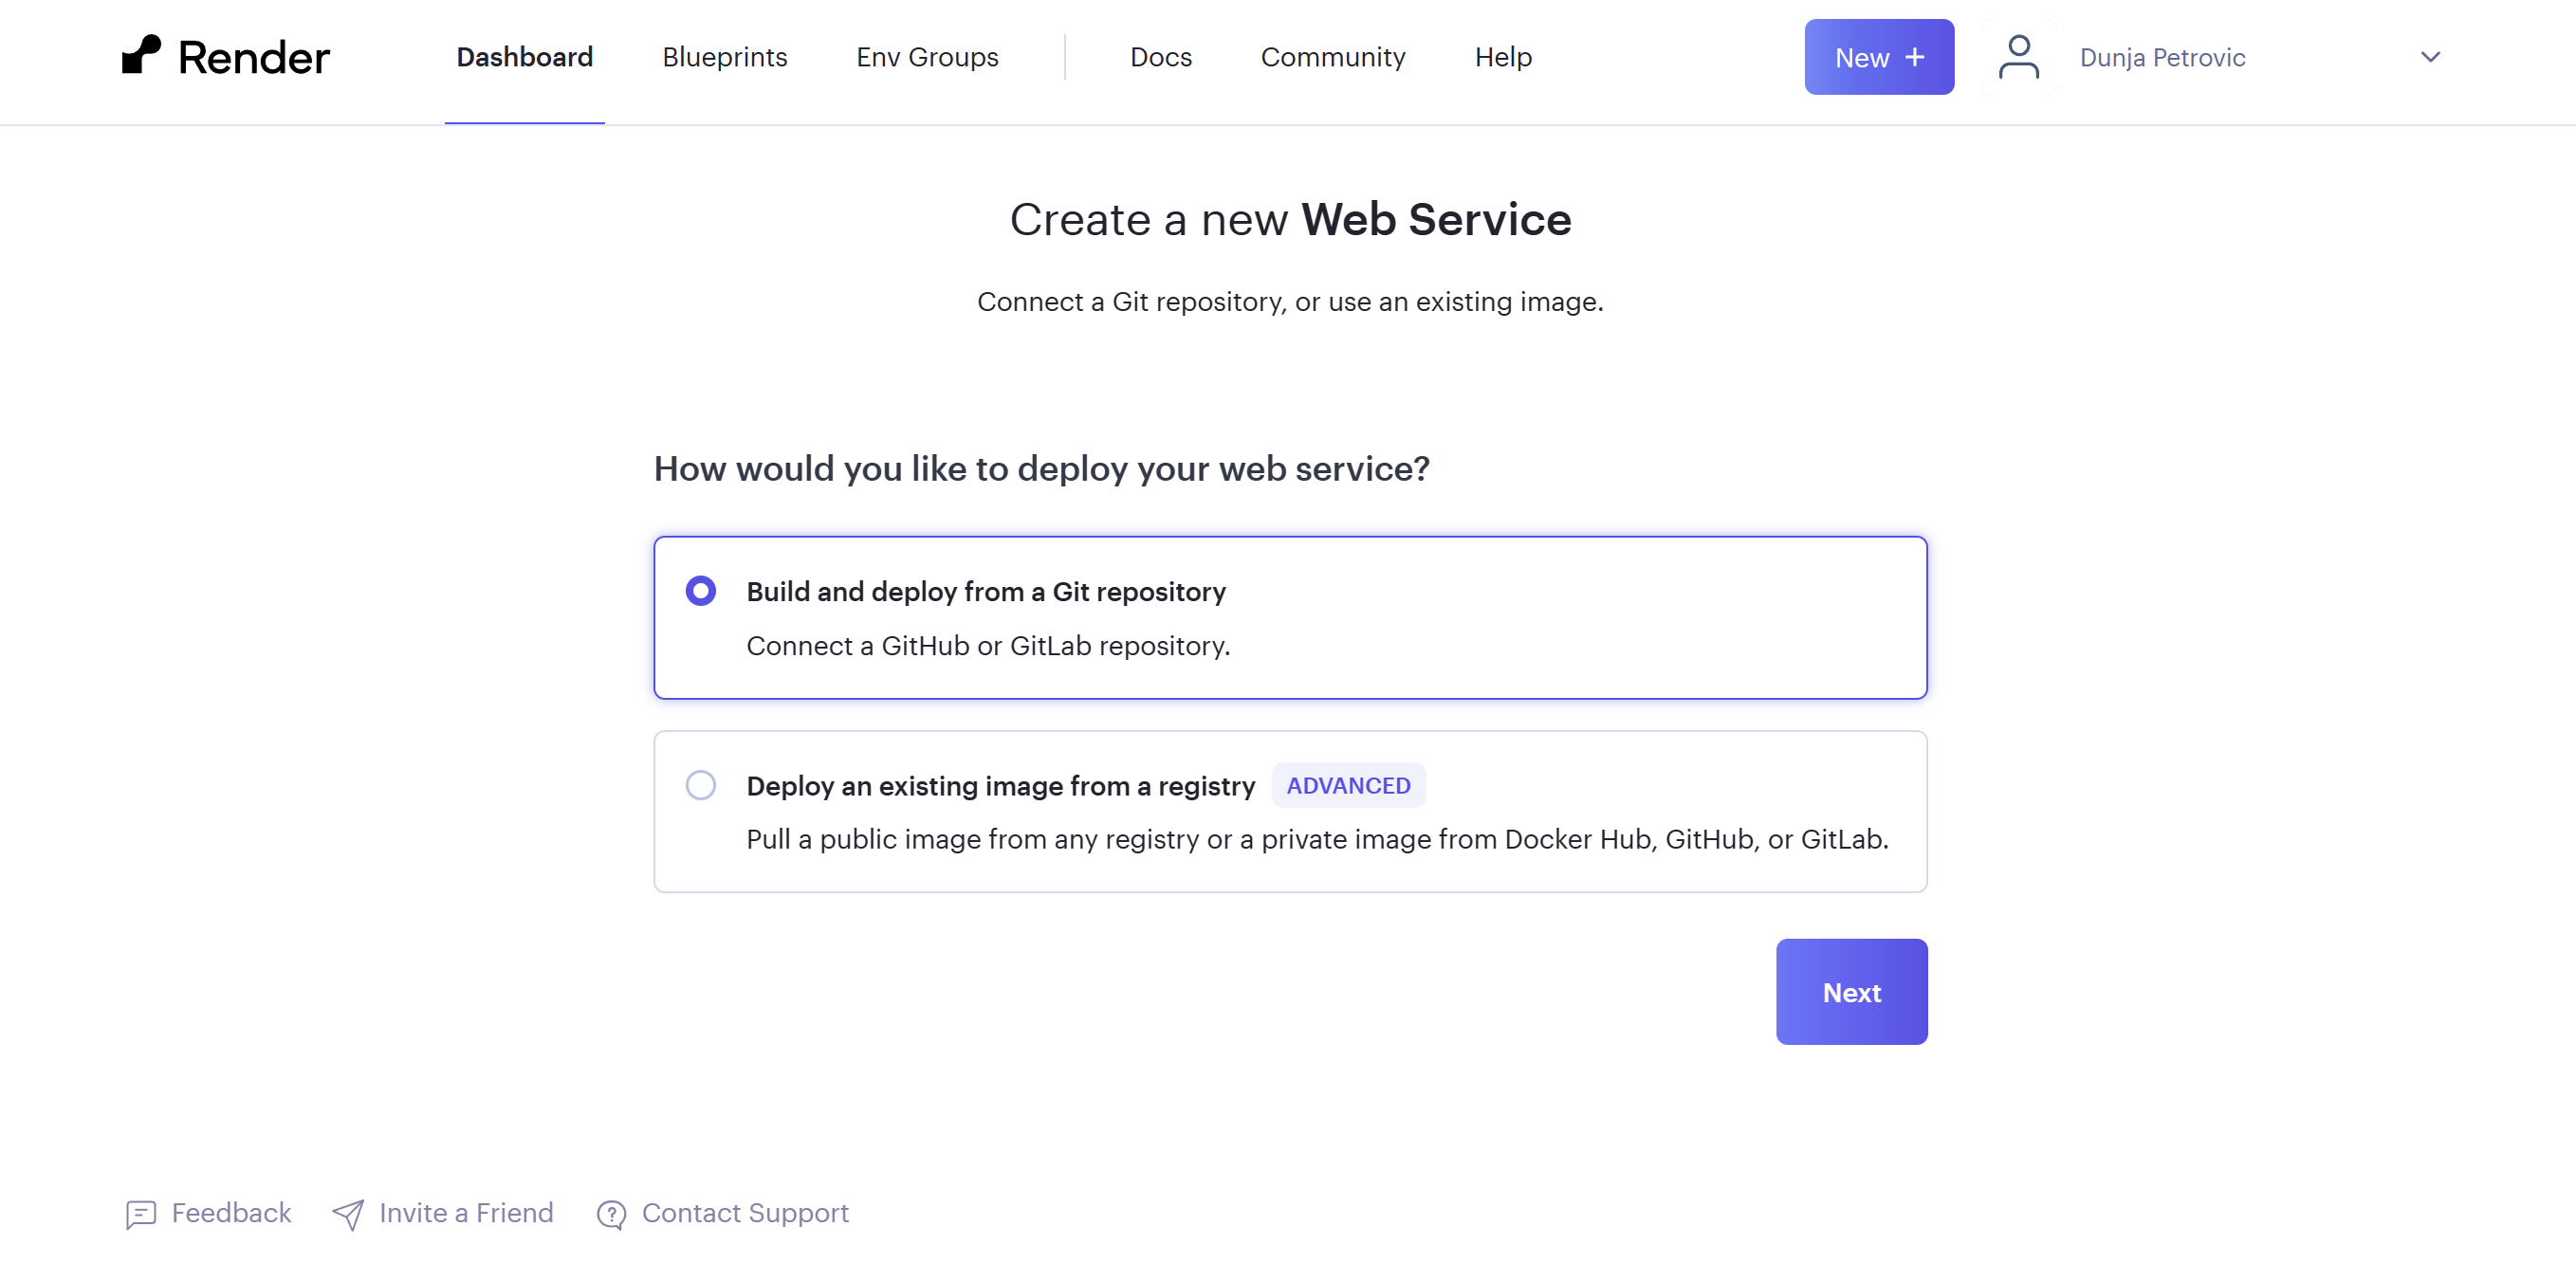
\includegraphics[scale=0.4]{slike/Render_ODABIR_OPCIJE.PNG} %veličina slike u odnosu na originalnu datoteku i pozicija slike
			\centering
			\caption{Odabir opcije dodavanja iz postojećeg GitHub repozitorija}
			\label{Odabir opcije dodavanja iz postojećeg GitHub repozitorija}
		\end{figure}
		
	    Nakon povezivanja Render računa s GitHub računom, slijedi odabir repozitorija, kako je prikazano na slici ispod. Mi smo odabrali repozitorij ljubo9/30bodova.
	    
	    	\begin{figure}[H]
			\includegraphics[scale=0.4]{slike/Render_ODABIR_REPOZITORIJA.PNG} %veličina slike u odnosu na originalnu datoteku i pozicija slike
			\centering
			\caption{Odabir repozitorija}
			\label{Odabir repozitorija}
		\end{figure}
		
		Odabir repozitorija slijedi podešavanje svih potrebnih opcija kako bi se Spring Boot poslužitelj ispravno pokrenuo. Na slici ispod prikazane su postavke koje je potrebno postaviti za ispravan rad poslužitelja.
		
		\begin{figure}[H]
			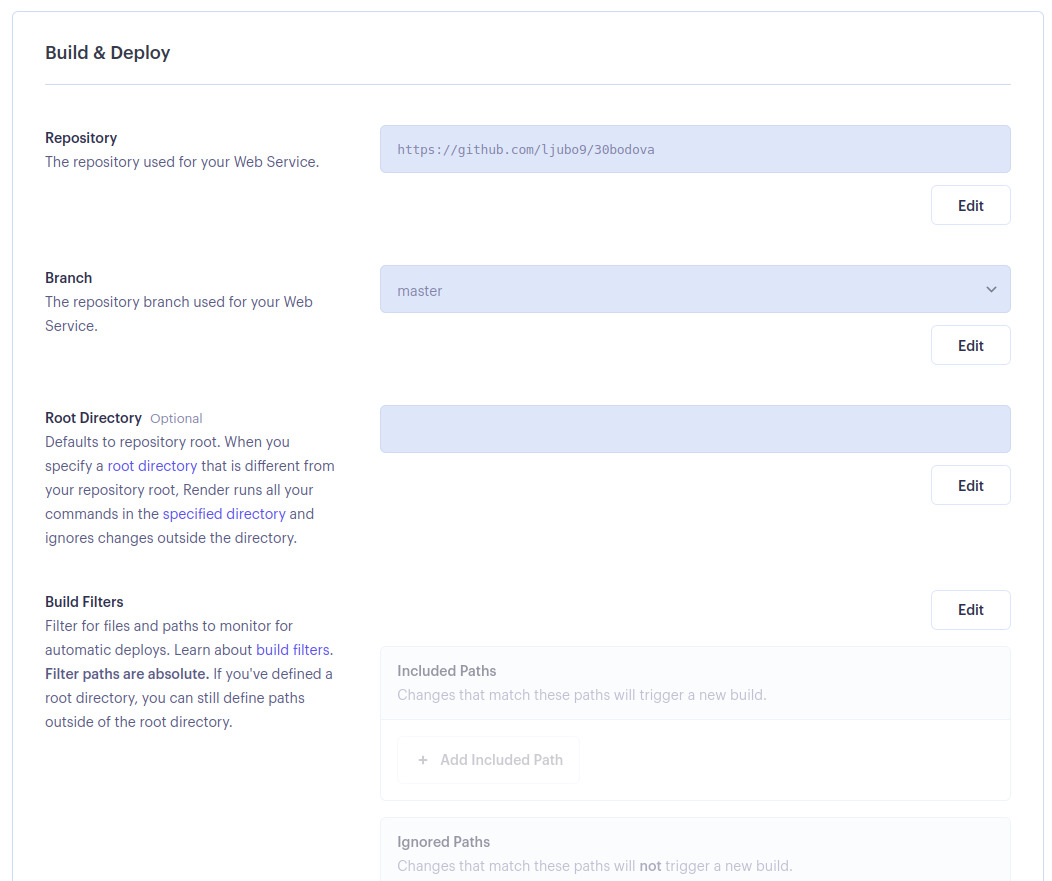
\includegraphics[scale=0.4]{slike/Render_BACKEND_1.JPG} %veličina slike u odnosu na originalnu datoteku i pozicija slike
			\centering
			\caption{Postavke za postavljanje Spring Boot poslužitelja, 1. dio}
			\label{Postavke za postavljanje Spring Boot poslužitelja, 1. dio}
		\end{figure}
		
		Na gornjoj je slici još jednom vidljiv odabrani repozitorij, odabrana grana (mi smo odabrali granu "master") i korijenski direktorij (nama to nije bilo važno pa smo ga ostavili praznog).
		
		Na slici ispod može se vidjeti drugi dio potrebnih postavki za postavljanje Spring Boot poslužitelja.
		
				\begin{figure}[H]
			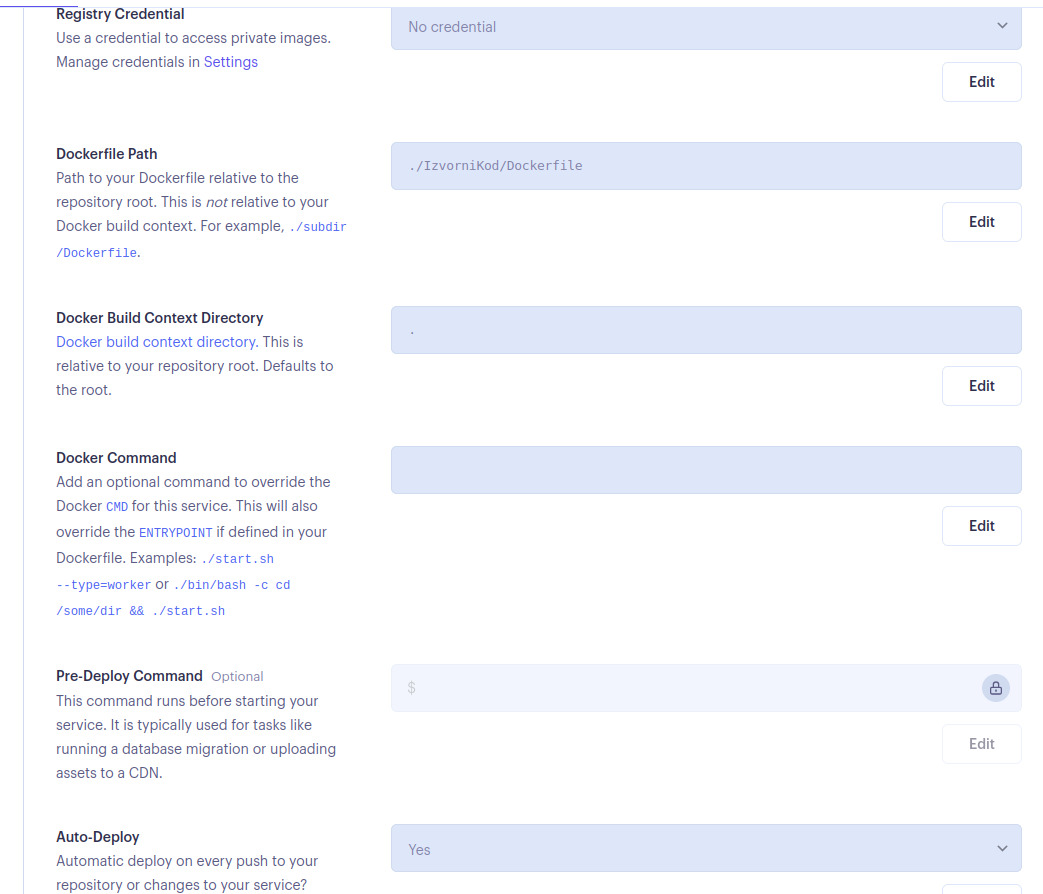
\includegraphics[scale=0.4]{slike/Render_BACKEND_2.JPG} %veličina slike u odnosu na originalnu datoteku i pozicija slike
			\centering
			\caption{Postavke za postavljanje Spring poslužitelja, 2. dio}
			\label{Postavke za postavljanje Spring poslužitelja, 2. dio}
		\end{figure}
		
		Ono što je bilo važno podesiti je bila lokacija Dockerfile-a, koju smo mi podesili na ./IzvorniKod/Dockerfile. Usto, označili smo i opciju "Auto-Deploy" s "Yes" , tako da se svaki put kada se neka nova izmjena napravi u kodu, Spring Boot poslužitelj se iznova "deploy-a". Time je deploy Spring Boot poslužitelja priveden kraju.
		
	\textbf{Postavljanje React web aplikacije} \\
	Kao i postavljanje Spring Boot poslužitelja, postavljanje React web aplikacije na Render je izrazito jednostavno. Svi koraci do podešavanja postavki za ispravan rad React web aplikacije jednaki su kao za postavljanje Spring Boot poslužitelja: dodavanje novog "web service-a", odabir opcije spajanja s GitHub repozitorijem, spajanje sa željenim GitHub računom te odabir GitHub repozitorija u kojem se nalazi projekt.
	
	Ono što se razlikuje je podešavanje ispravnih postavki za pokretanje React web aplikacije. Na slici ispod prikazane su potrebne postavke.
	
		\begin{figure}[H]
			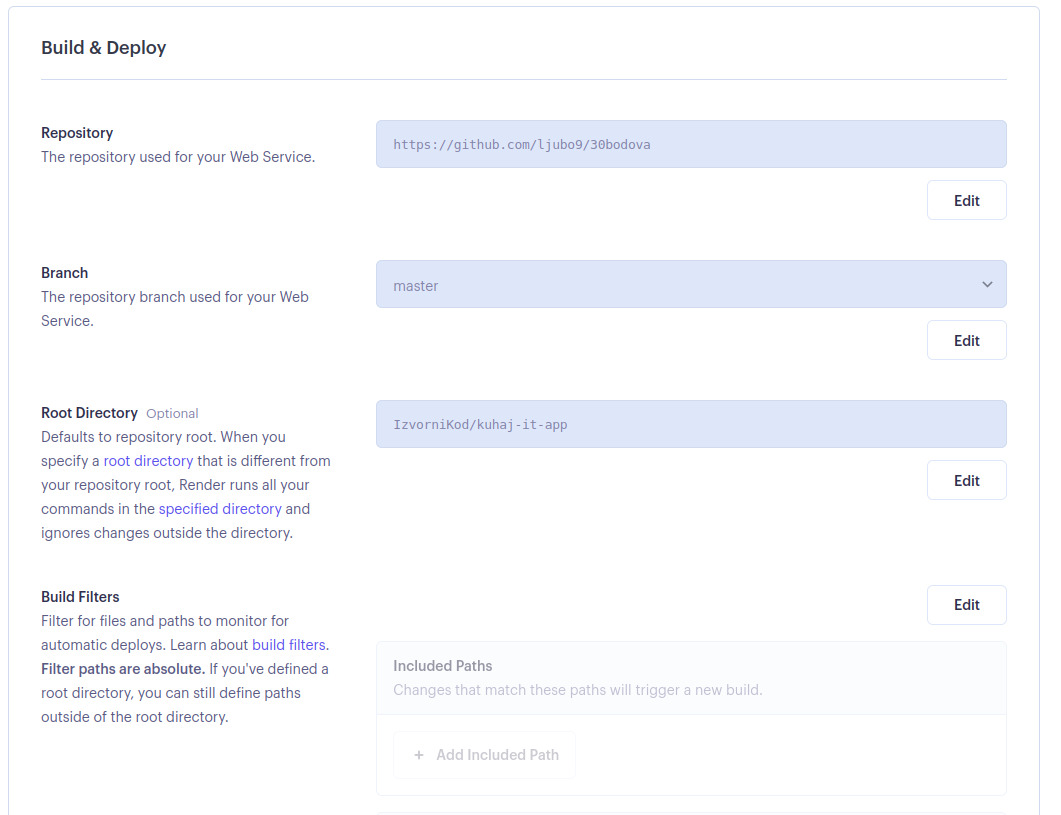
\includegraphics[scale=0.4]{slike/Render_FRONTEND_1.JPG} %veličina slike u odnosu na originalnu datoteku i pozicija slike
			\centering
			\caption{Postavke za postavljanje React web aplikacije, 1. dio}
			\label{Postavke za postavljanje React web aplikacije, 1. dio}
		\end{figure}
		
	Odabrani repozitorij isti je kao za postavljanje Spring Boot poslužitelja, kao i odabrana grana repozitorija.
	Za razliku od postavljanja Spring Boot poslužitelja, ovdje smo za korijenski direktorij odabrali direktorij IzvorniKod/kuhaj-it-app. Drugi dio potrebnih postavki prikazan je na slici ispod.
	
			\begin{figure}[H]
			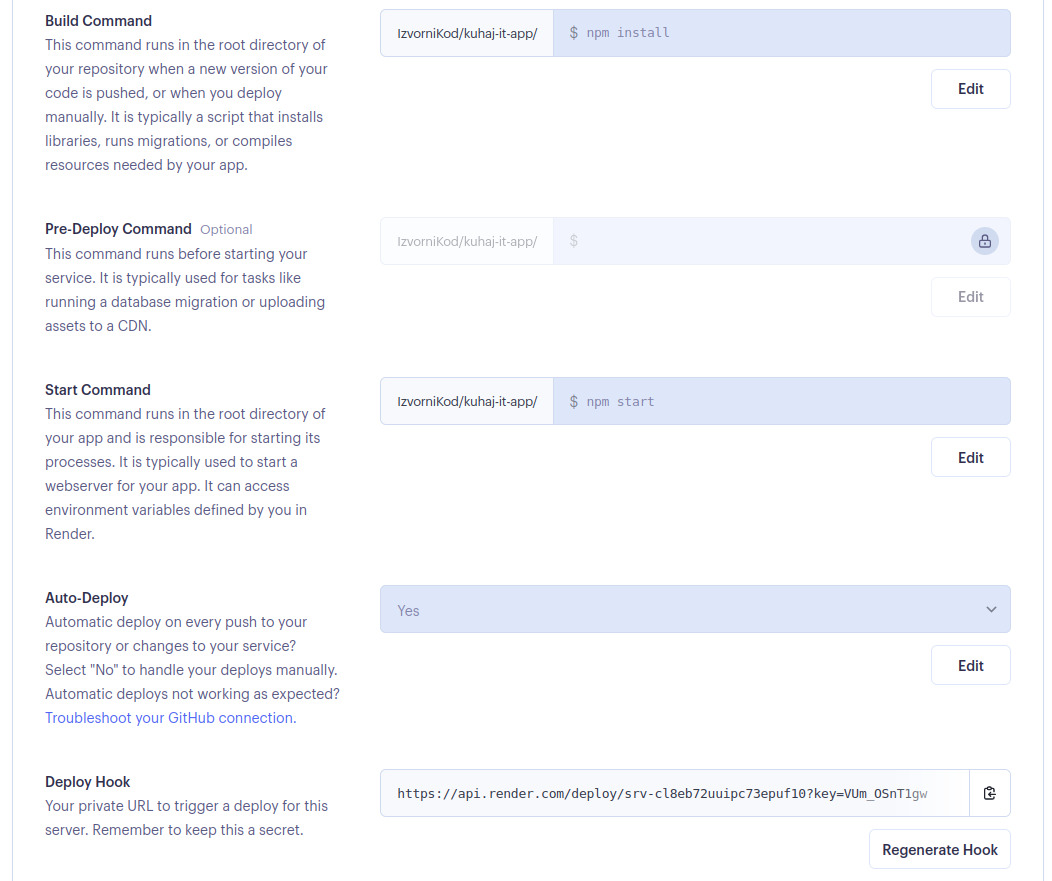
\includegraphics[scale=0.4]{slike/Render_FRONTEND_2.JPG} %veličina slike u odnosu na originalnu datoteku i pozicija slike
			\centering
			\caption{Postavke za postavljanje React web aplikacije, 2. dio}
			\label{Postavke za postavljanje React web aplikacije, 2. dio}
		\end{figure}
		
		Na gornjoj je slici vidljivo da smo za "naredbu izgradnje", naredbu koja će instalirati sve biblioteke, pokrenuti migracije i kompajlirati sve potrebno za ispravan rad naše React web aplikacije, odabrali naredbu "npm install".
		Ono što je još trebalo podesiti je naredba pokretanja, koju smo podesili na "npm start".
		Isto kao i kod podešavanja Spring Boot poslužitelja, odabrali smo opciju Auto-Deploy.
	
		
	
	
	
		
		
		
		
		
		
		
		
		 
		
		
	    
	    
		
		
		
		
		
		
		
			
			\eject 